% Dessin dans le plan d'un ouvert V_epsilon, x^*(0)

\begin{figure}[!h]
  \begin{center}
    \caption{Exemple d'ouvert $V_{\varepsilon, x^*}(0)$ dans le plan}%
    \label{w:ill}
    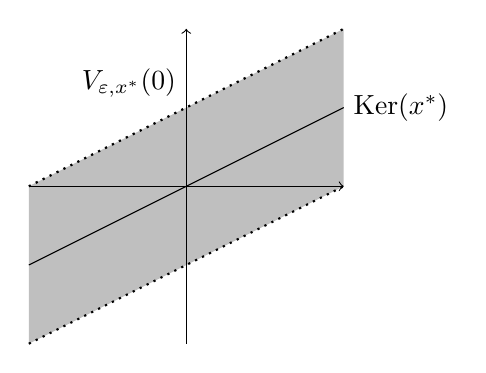
\begin{tikzpicture}
      \draw [->] (0, -2) -- (0, 2);
      \draw [->] (-2, 0) -- (2, 0);
      \draw (-2, -1) -- (2, 1) node[right] {$\mathrm{Ker}(x^*)$};
      \fill [black, nearly transparent] %
            (-2, -2) -- (-2, 0) -- (2, 2) -- (2, 0) -- cycle;
      \draw [dotted, thick] (-2, 0)  -- (0, 1)%
            node[above left] {$V_{\varepsilon, x^*}(0)$}-- (2, 2);
      \draw [dotted, thick] (-2, -2) -- (2, 0);
    \end{tikzpicture}
\end{center}
\end{figure}